\begin{figure*}[ht]
    \centering
    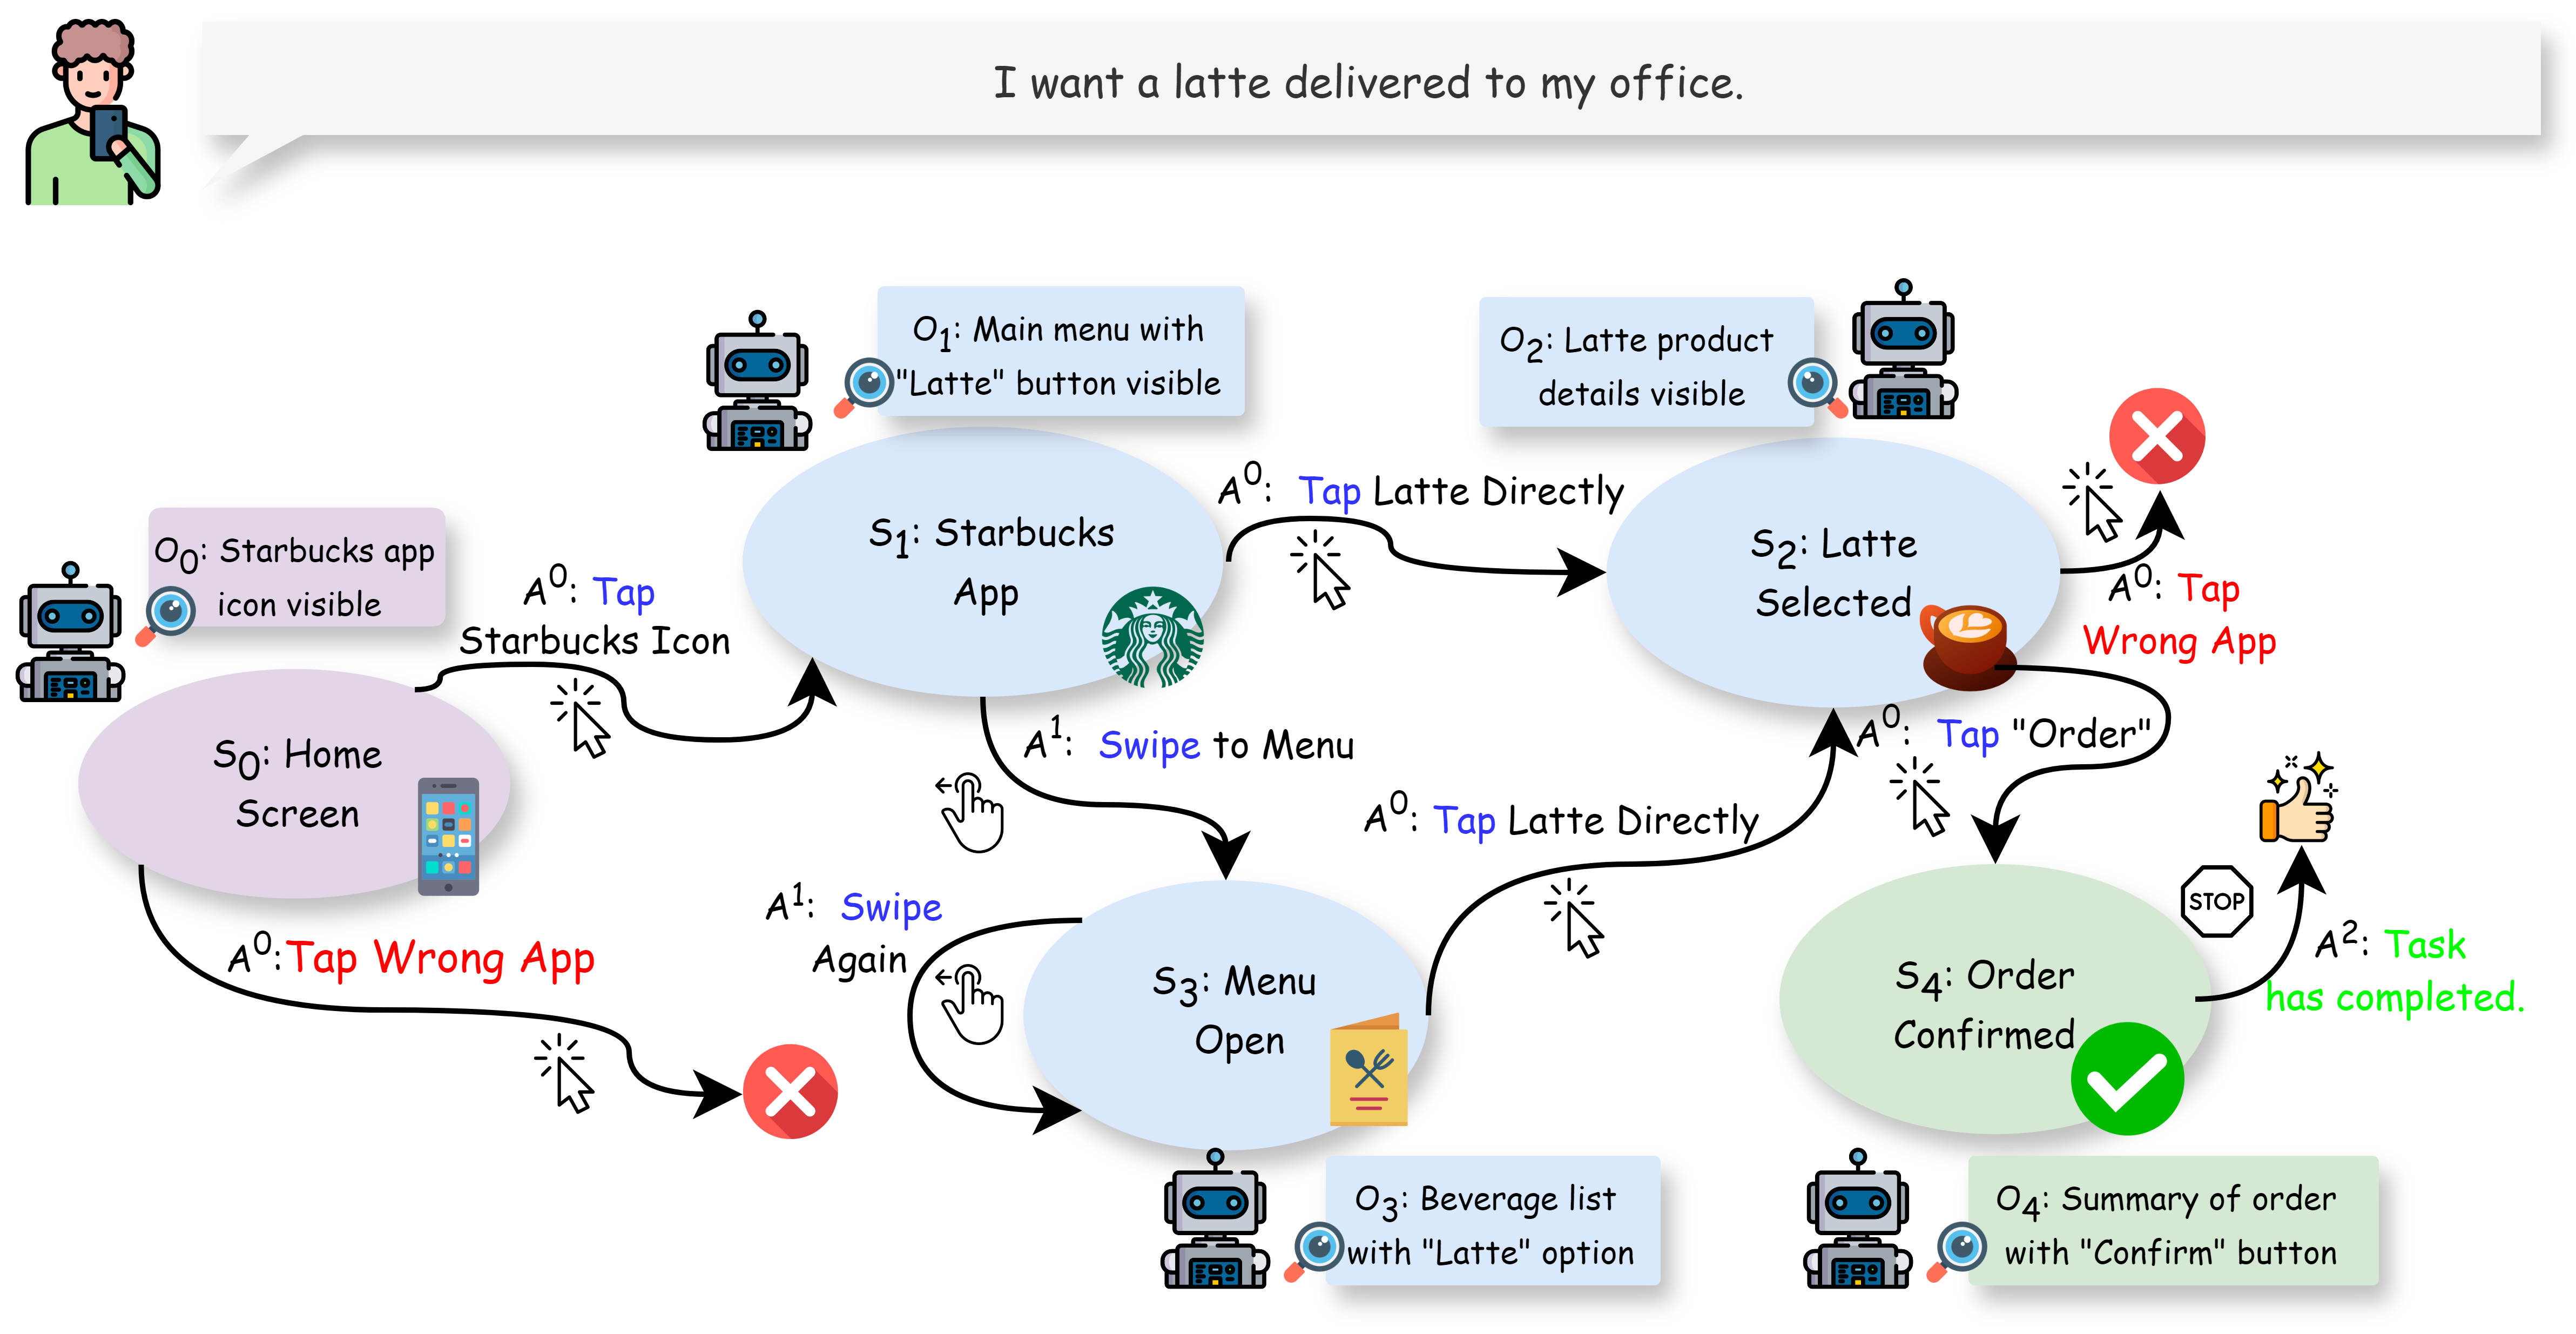
\includegraphics[width=0.95\textwidth]{figures/basic_pipline_mdp.drawio.png}
    \caption{POMDP model for ordering a latte. Each circle represents a state (e.g., Home Screen, App Homepage, Latte Details Page, Customize Order, Order Confirmation, Order Complete). The agent starts at the initial state $S_0$ (Home Screen) and makes decisions at each step (e.g., tapping the Starbucks app icon, selecting the "Latte" button, viewing latte details). Due to partial observability, the agent receives limited information at each decision point (e.g., $O_0$: Starbucks app icon visible, $O_1$: "Latte" button visible, $O_2$: Latte product details visible). Some actions correctly advance towards the goal, while others may cause errors requiring corrections. The final goal is to confirm the order.}
    \label{fig:basic_pipline_mdp}
\end{figure*}

\section{Frameworks and Components of Phone GUI Agents}
\label{sec:frameworks}

MLLM-powered phone GUI agents can be designed using different architectural paradigms and components, ranging from straightforward, single-agent systems~\cite{wang2023enabling,wen2023droidbot,wen2024autodroid,zhang2023appagent,wang2024mobileagentv1} to more elaborate multi-agent~\cite{wang2024mobileagentv2,zhang2024mobileexperts,zhang2024dynamic} or multi-stage~\cite{zheng2024gpt,gou2024navigating,hoscilowicz2024clickagent} approaches. A fundamental scenario involves a \textit{single agent} that operates incrementally, without precomputing an entire action sequence from the outset. Instead, the agent continuously observes the \textbf{dynamically changing} mobile environment—where available UI elements, device states, and relevant contextual factors may shift in unpredictable ways—and cannot be exhaustively enumerated in advance. As a result, the agent must adapt its strategy \textbf{step-by-step}, making decisions based on the current situation rather than following a fixed plan. This \textbf{iterative} decision-making process can be effectively modeled using a \textbf{Partially Observable Markov Decision Process (POMDP)}, a well-established framework for handling sequential decision-making under uncertainty~\cite{monahan1982state,spaan2012partially}. By modeling the task as a POMDP, we capture its dynamic nature, the impossibility of pre-planning all actions, and the necessity of adjusting the agent’s approach at each decision point.

As illustrated in Figure~\ref{fig:basic_pipline_mdp}, consider a simple example: the agent’s goal is to order a latte through the Starbucks app. The app’s interface may vary depending on network latency, promotions displayed, or the user’s last visited screen. The agent cannot simply plan all steps in advance; it must observe the current screen, identify which UI elements are present, and then choose an action (like tapping the Starbucks icon, swiping to a menu, or selecting the latte). After each action, the state changes, and the agent re-evaluates its options. This dynamic, incremental decision-making is precisely why POMDPs are a suitable framework. In the POMDP formulation for phone automation:



\noindent\textbf{States ($S$).}
At each decision point, the agent’s perspective is described as a \textit{state}, a comprehensive snapshot of all relevant information that could potentially influence the decision-making process. This state encompasses the current \textbf{UI information} (e.g., screenshots, UI trees, OCR-extracted text, icons), the \textbf{phone’s own status} (network conditions, battery level, location), and the \textbf{task context} (the user’s goal—“order a latte”—and the agent’s progress toward it). The state $S_t$ represents the complete, underlying situation of the environment at time $t$, which may not be directly observable in its entirety.


\noindent\textbf{Actions ($A$).}
Given the state $S_t$ at time $t$, the agent selects from available actions (taps, swipes, typing text, launching apps) that influence the subsequent state.  The details of how phone GUI agents make decisions are introduced in \S\ \ref{subsec:brain}, and the design of the action space is discussed in \S\ \ref{subsec:action}.


\noindent\textbf{Transition Dynamics ($P(s'|s,a)$).}
When the agent executes an action $a_t$ at time $t$, it leads to a new state $S_{t+1}$. Some transitions may be deterministic (e.g., tapping a known button reliably opens a menu), while others are uncertain (e.g., network delays, unexpected pop-ups). Mathematically, we have the transition probability $P(s'|s,a)$ which describes the likelihood of transitioning from state $S_t$ to state $S_{t+1}$ given action $a_t$.



\noindent\textbf{Observations ($O$).}
The agent receives \textit{observations} $O_t$ at time $t$ which are partial and imperfect reflections of the true state $S_t$. In the phone automation context, these observations could be, for example, a glimpse of the visible UI elements (not the entire UI tree), a brief indication of the network status (such as a signal icon without detailed connection parameters), or a partial view of the battery level indicator. These observations $O_t$ provide the agent with some, but not all, of the information relevant to the state $S_t$. The agent must infer and make decisions based on these limited observations, attempting to reach the desired goal state despite the partial observability. The details of phone GUI agent perception are discussed in \S\ \ref{subsec:perception}.


Under this POMDP-based paradigm, the agent aims to make decisions that lead to the goal state by observing the current state and choosing appropriate actions. It continuously re-evaluates its strategy as conditions evolve, promoting real-time responsiveness and dynamic adaptation. The agent \textbf{observes the state $S_t$ at time $t$, chooses an action $a_t$, and then based on the resulting observation $O_{t+1}$ and new state $S_{t+1}$}, refines its strategy.

As illustrated in Figure~\ref{fig:phone_agent_framework}, frameworks of phone GUI agents aim to integrate perception, reasoning, and action capabilities into cohesive agents that can interpret user intentions, understand complex UI states, and execute appropriate operations within mobile environment. By examining these frameworks, we can identify best practices, guide future advancements, and choose the right approach for various applications and contexts.

\begin{figure*}[ht]
    \centering
    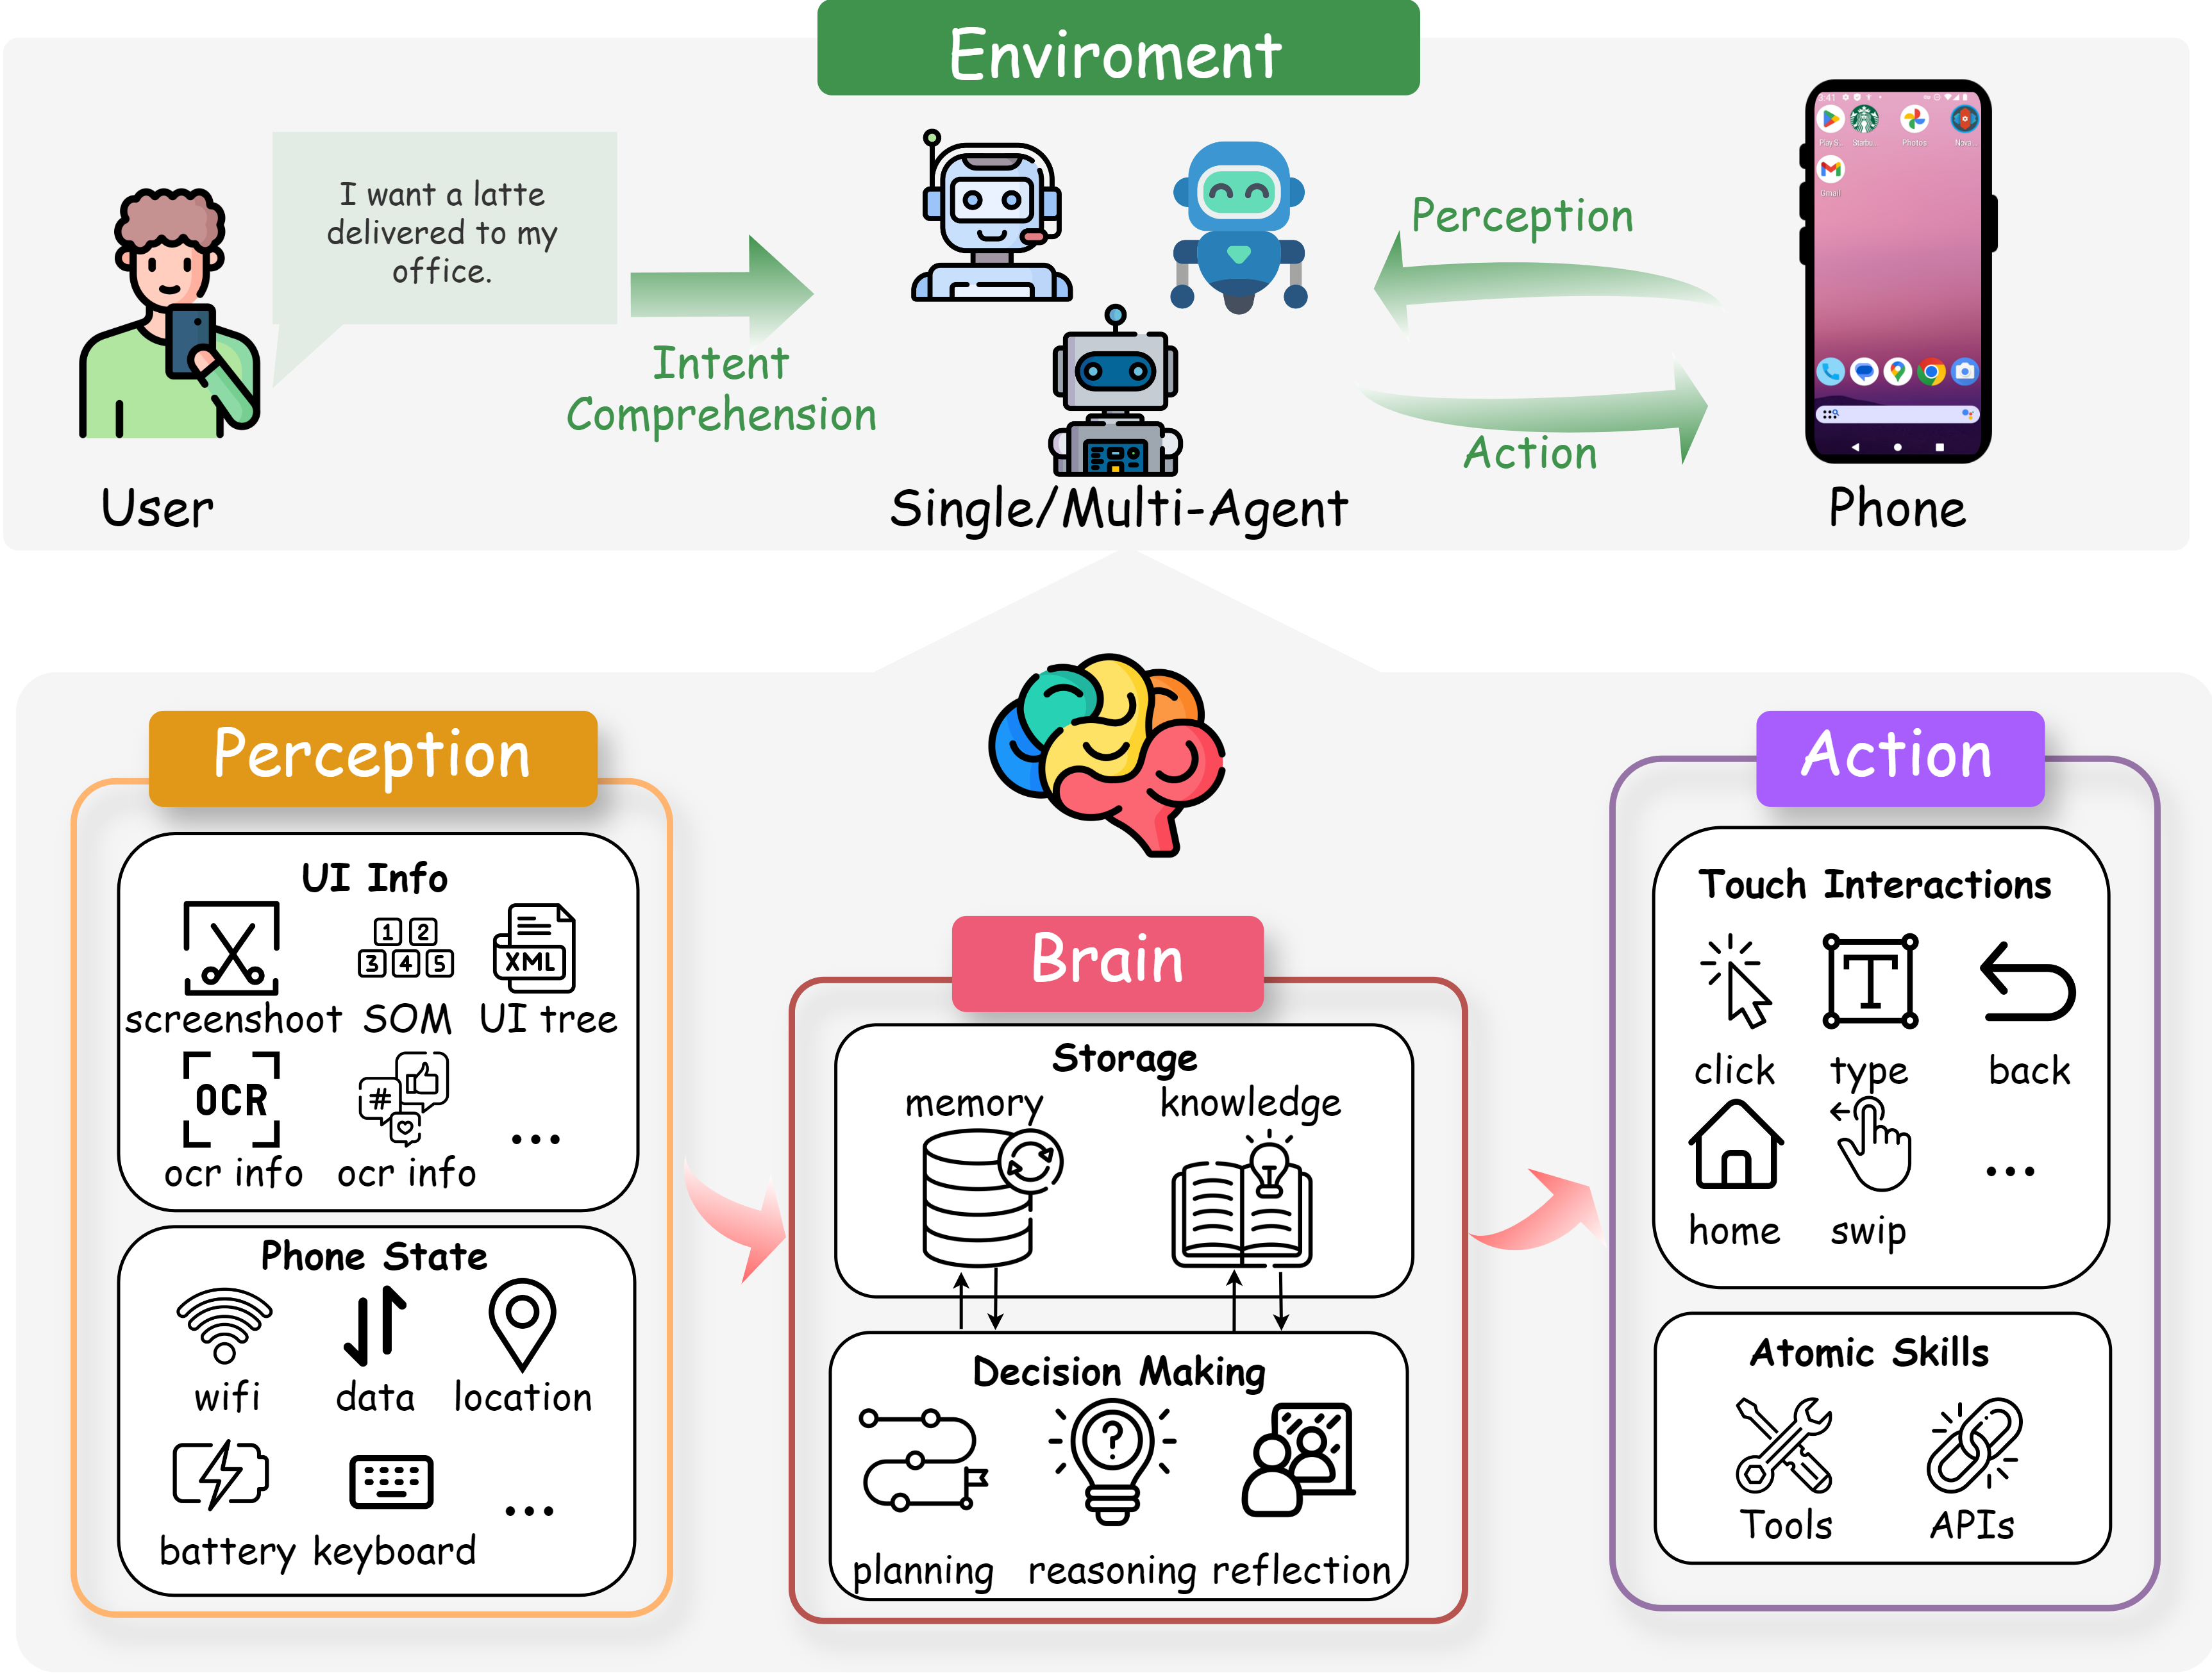
\includegraphics[width=0.95\textwidth]{figures/phone_agent_framework.drawio.png}
    \caption{Overview of MLLM-powered phone GUI agent framework. The user's intent, expressed through natural language, is mapped to UI operations. By perceiving UI information and phone state(\S\ref{subsec:perception}) , the agent leverages stored knowledge and memory to plan, reason, and reflect (\S\ref{subsec:brain}) . Finally, it executes actions to fulfill the user's goals(\S\ref{subsec:action}).}
    \label{fig:phone_agent_framework}
\end{figure*}

To address limitations in adaptability and scalability, \S\ref{subsec:mult_agent} introduces multi-agent frameworks, where specialized agents collaborate, enhance efficiency, and handle more diverse tasks in parallel. Finally, \S\ref{subsec:plan_then_act} presents the Plan-Then-Act Framework, which explicitly separates the planning phase from the execution phase. This approach allows agents to refine their conceptual plans before acting, potentially improving both accuracy and robustness.


\subsection{Perception in Phone GUI Agents}
\label{subsec:perception}

Perception is a fundamental component of the basic framework for MLLM-powered phone GUI agents. It is responsible for capturing and interpreting the state of the mobile environment, enabling the agent to understand the current context and make informed decisions. In the overall pipeline, perception serves as the initial step in the POMDP, providing the necessary input for the reasoning and action modules to operate effectively.

\subsubsection{UI Information Perception}

UI information is crucial for agents to interact seamlessly with the mobile interface. It can be further categorized into UI tree-based and screenshot-based approaches, supplemented by techniques like Set-of-Marks (SoM) and Icon \& OCR enhancements.


\noindent\textbf{UI tree}
is a structured, hierarchical representation of the UI elements on a mobile screen~\cite{medhi2013comparison,rasanen2015sequence}. Each node in the UI tree corresponds to a UI component, containing attributes such as class type, visibility, and resource identifiers.\footnote{\href{https://developer.android.com/reference/android/view/View}{https://developer.android.com/reference/android/view/View}.} Early datasets like PixelHelp~\cite{li2020PixelHelp}, MoTIF~\cite{burns2021motif}, and UIBert~\cite{bai2021uibert} utilized UI tree data to enable tasks such as mapping natural language instructions to UI actions and performing interactive visual environment interactions.
DroidBot-GPT~\cite{wen2023droidbot} was the first work to investigate how pre-trained language models can be applied to app automation without modifying the app or the model. DroidBot-GPT uses the UI tree as its primary perception information. The challenge lies in converting the structured UI tree into a format that LLMs can process effectively. DroidBot-GPT addresses this by transforming the UI tree into natural language sentences. Specifically, it extracts all user-visible elements, generates prompts like ``A view \textless name\textgreater that can...'' for each element, and combines them into a cohesive description of the current UI state. This approach mitigates the issue of excessively long and complex UI trees by presenting the information in a more natural and concise format suitable for LLMs.
Subsequent developments, such as Enabling Conversational Interaction~\cite{wang2023enabling} and AutoDroid~\cite{wen2024autodroid}, further refined this approach by representing the view hierarchy as HTML. Enabling Conversational Interaction introduces a method to convert the view hierarchy into HTML syntax, mapping Android UI classes to corresponding HTML tags and preserving essential attributes such as class type, text, and resource identifiers. This representation aligns closely with the training data distribution of LLMs, enhancing their ability to perform few-shot learning and improving overall UI understanding. AutoDroid extends this work by developing a GUI parsing module that converts the GUI into a simplified HTML representation using specific HTML tags like \textless button\textgreater, \textless checkbox\textgreater, \textless scroller\textgreater, \textless input\textgreater, and \textless p\textgreater. Additionally, AutoDroid implements automatic scrolling of scrollable components to ensure that comprehensive UI information is available to the LLM, thereby enhancing decision-making accuracy and reducing computational overhead.
Furthermore, LLMPA~\cite{guan2023intelligent} employs object detection models to comprehend page layouts and optimizes the grouping of UI elements for potential actions. This approach reduces redundant information in the UI tree, thereby enhancing the accuracy and speed of decision making. Similar to this approach, the TOL Agent~\cite{fan2024readpointedlayoutawaregui} introduces a variant of the UI tree, known as the Hierarchical Layout Tree, to represent the hierarchical layout of screen captures. In this tree, nodes represent different levels of regions. This structure, combined with a trained DINO model, aids in generating more accurate screen descriptions for MLLM.


\noindent\textbf{Screenshots}
provide a visual snapshot of the current UI, capturing the appearance and layout of UI elements. Unlike UI trees, which require API access and can become unwieldy with complex hierarchies, screenshots offer a more flexible and often more comprehensive representation of the UI. Additionally, UI trees present challenges such as missing or overlapping controls and the inability to directly reference UI elements programmatically, making screenshots a more practical and user-friendly alternative for quickly assessing and sharing the state of a user interface.
Auto-GUI~\cite{zhang2023youautoui} introduced a multimodal agent that relies on screenshots for GUI control, eliminating the dependency on UI trees. This approach allows the agent to interact with the UI directly through visual perception, enabling more natural and human-like interactions. Auto-GUI employs a chain-of-action technique that uses both previously executed actions and planned future actions to guide decision-making, achieving high action type prediction accuracy and efficient task execution.
Following Auto-GUI, a series of multimodal solutions emerged, including MM-Navigator~\cite{yan2023gpt}, CogAgent~\cite{hong2024cogagent}, AppAgent~\cite{zhang2023appagent}, VisionTasker~\cite{song2024visiontasker}, MobileGPT~\cite{lee2023exploremobilegpt}, GUI Narrator~\cite{wu2024gui}, MobileVLM~\cite{wu2024mobilevlm}, AdaptAgent~\cite{verma2024adaptagent}, WebVoyager~\cite{he2024webvoyager} and Steward~\cite{tang2024steward}. These frameworks leverage screenshots in combination with supplementary information to enhance UI understanding and interaction capabilities.



\noindent\textbf{Set-of-Mark (SoM)}
is a prompting technique used to annotate screenshots with OCR, icon, and UI tree information, thereby enriching the visual data with textual descriptors\cite{yang2023setofmark}. For example, MM-Navigator~\cite{yan2023gpt} uses SoM to label UI elements with unique identifiers, allowing the LLM to reference and interact with specific components more effectively. This method has been widely adopted in subsequent works such as AppAgent~\cite{zhang2023appagent}, VisionDroid~\cite{liu2024vision}, OmniParser~\cite{lu2024omniparser} and VisualWebArena~\cite{koh2024visualwebarena}, which utilize SoM to enhance the agent's ability to interpret and act upon UI elements based on visual, textual, and structural cues.
% add VisualWebArena


\noindent\textbf{Icon \& OCR enhancements}
provide additional layers of information that complement the visual data, enabling more precise action decisions. For instance, Mobile-Agent-v2~\cite{wang2024mobileagentv2} integrates OCR and icon data with screenshots to provide a richer context for the LLM, allowing it to interpret and execute more complex instructions that require understanding both text and visual icons. Icon \& OCR enhancements are employed in various works, including VisionTasker~\cite{song2024visiontasker}, MobileGPT~\cite{lee2023exploremobilegpt},  OmniParser~\cite{lu2024omniparser}, and WindowsAgentArena~\cite{bonatti2024windows}, to improve the accuracy and reliability of phone GUI agents.


\subsubsection{Phone State Perception}

Phone state information, such as keyboard status and location data, further contextualizes the agent's interactions. For example, Mobile-Agent-v2~\cite{wang2024mobileagentv2} uses keyboard status to determine when text input is required. Location data, while not currently utilized, represents a potential form of phone state information that could be used to recommend nearby services or navigate to specific addresses. This additional state information enhances the agent's ability to perform context-aware actions, making interactions more intuitive and efficient.



The perception information gathered through UI trees, screenshots, SoM, OCR, and phone state is converted into prompt tokens that the LLM can process. This conversion is crucial for enabling seamless interaction between the perception module and the reasoning and action modules. Detailed methodologies for transforming perception data into prompt formats are discussed in \S\ \ref{subsec:prompt_engineering}.

\subsection{Brain in Phone GUI Agents}
\label{subsec:brain}

The brain of an LLM-based phone automation agent is its cognitive core, primarily constituted by a  LLM. The LLM serves as the agent's reasoning and decision-making center, enabling it to interpret inputs, generate appropriate responses, and execute actions within the mobile environment~\cite{ge2023llm,mei2024aios}. Leveraging the extensive knowledge embedded within LLMs, agents benefit from advanced language understanding, contextual awareness, and the ability to generalize across diverse tasks and scenarios.

\subsubsection{Storage}

Storage encompasses both memory and knowledge, which are critical for maintaining context and informing the agent's decision-making processes.


\noindent\textbf{Memory}
refers to the agent's ability to retain information from past interactions with users and the environment~\cite{xi2023rise}. This is particularly useful for cross-application operations, where continuity and coherence are essential for completing multi-step tasks. For example, Mobile-Agent-v2~\cite{wang2024mobileagentv2} integrates a memory unit that records task-related focus content from historical screens. This memory is accessed by the decision-making module when generating operations, ensuring that the agent can reference and update relevant information dynamically.
The Self-MAP framework~\cite{deng2024multi} establishes a memory repository based on the history of conversational interactions. It utilizes a multifaceted matching approach to retrieve the top-K memory snippets that are semantically relevant to the current dialogue state and have similar trajectories. This assists the agent in effectively utilizing limited context space during multi-turn interactions, thereby enhancing its ability to comprehend and execute user instructions.



\noindent\textbf{Knowledge}
pertains to the agent's understanding of phone automation tasks and the functionalities of various apps. This knowledge can originate from multiple sources:

\begin{itemize}
    \item \textbf{Pre-trained Knowledge.} LLMs are inherently equipped with a vast amount of general knowledge, including common-sense reasoning and familiarity with programming and markup languages such as HTML. This pre-existing knowledge allows the agent to interpret and generate meaningful actions based on the UI representations.
    
    \item \textbf{Domain-Specific Training.} Some agents enhance their knowledge by training on phone automation-specific datasets. Works such as Auto-GUI~\cite{zhang2023youautoui}, CogAgent~\cite{hong2024cogagent}, ScreenAI~\cite{baechler2024screenai}, CoCo-agent~\cite{ma2024coco}, and Ferret-UI~\cite{you2024ferret} have trained LLMs on datasets tailored for mobile UI interactions, thereby improving their capability to understand and manipulate mobile interfaces effectively. For a more detailed discussion of knowledge acquisition through model training, see \S\ \ref{subsec:training_based}.

    
    \item \textbf{Knowledge Injection.} Agents can enhance their decision-making by incorporating knowledge derived from exploratory interactions and stored contextual information. This involves utilizing data collected during offline exploration phases or from observed human demonstrations to inform the LLM's reasoning process. For instance, AutoDroid~\cite{wen2024autodroid} explores app functionalities and records UI transitions in a UI Transition Graph (UTG) memory, which are then used to generate task-specific prompts for the LLM. Similarly, AppAgent~\cite{zhang2023appagent} compiles knowledge from autonomous interactions and human demonstrations into structured documents, enabling the LLM to make informed decisions based on comprehensive UI state information and task requirements.
    AppAgent v2~\cite{li2024appagentv2} introduces a more efficient mechanism for knowledge base construction and updating. It leverages Retrieval-Augmented Generation (RAG) technology to achieve real-time dynamic updates of knowledge base information. This significantly enhances the agent's adaptability in new environments.AppAgentX~\cite{li2024appagentx} introduces an evolutionary mechanism that enables dynamic learning from past interactions and replaces inefficient low-level operations with high-level actions. Other similar works include AdaptAgent~\cite{verma2024adaptagent}, Mobile-Agent-V~\cite{wang2025mobileagentv}, LearnAct~\cite{liu2025learnact} and others.
\end{itemize}

\subsubsection{Decision Making}

Decision Making is the process by which the agent determines the appropriate actions to perform based on the current perception and stored information~\cite{xi2023rise}. The LLM processes the input prompts, which include the current UI state, historical interactions from memory, and relevant knowledge, to generate action sequences that accomplish the assigned tasks.


\noindent\textbf{Planning}
involves devising a sequence of actions to achieve a specific task goal~\cite{song2023llm,xi2023rise}. Effective planning is essential for decomposing complex tasks into manageable steps and adapting to changes in the environment. For instance, Mobile-Agent-v2~\cite{wang2024mobileagentv2} incorporates a planning agent that generates task progress based on historical operations, ensuring effective operation generation by the decision agent. Additionally, approaches like Dynamic Planning of Thoughts (D-PoT) have been proposed to dynamically adjust plans based on environmental feedback and action history, significantly improving accuracy and adaptability in task execution~\cite{zhang2024dynamic}. Simultaneously, by reducing the number of calls to LLMs and employing a phased planning strategy, the agent can plan all actions in a given state at once, thereby enhancing planning efficiency~\cite{li2023zero}.



\noindent\textbf{Reasoning}
enables the agent to interpret and analyze information to make informed decisions~\cite{gandhi2024understanding,chen2024optimizing,plaat2024reasoning}. It involves understanding the context, evaluating possible actions, and selecting the most appropriate ones to achieve the desired outcome. By leveraging chain-of-thought(COT)~\cite{wei2022chain}, LLMs enhance their reasoning capabilities, allowing them to think step-by-step and handle intricate decision-making processes. This structured approach facilitates the generation of coherent and logical action sequences, ensuring that the agent can navigate complex UI interactions effectively.
The best-first tree search algorithm is utilized in real-world environments to iteratively construct, explore, and prune trajectory graphs, thereby enhancing the reasoning and decision-making capabilities of agents. A value function serves as a reward signal to guide agents in conducting efficient searches~\cite{koh2024tree}. Additionally, research indicates that LLMs to estimate the latent states of agents, in combination with reasoning methods, can further improve the agents' reasoning performance~\cite{bishop2024latent}.


\noindent\textbf{Reflection}
allows the agent to assess the outcomes of its actions and make necessary adjustments to improve performance~\cite{shinn2024reflexion}. It involves evaluating whether the executed actions meet the expected results and identifying any discrepancies or errors. For example, Mobile-Agent-v2~\cite{wang2024mobileagentv2} includes a reflection agent that evaluates whether the decision agent’s operations align with the task goals. If discrepancies are detected, the reflection agent generates appropriate remedial measures to correct the course of action. This continuous feedback loop enhances the agent's reliability and ensures that it can recover from unexpected states or errors during task execution. Furthermore, structured self-reflection identifies initial erroneous actions, which prevents agents from repeating the same mistakes. It also draws on reflective memory to avoid known unsuccessful actions~\cite{li2023zero}. Additionally, regular reflection through automated evaluation methods significantly enhances the performance of agents~\cite{pan2024autonomous,duan2024uicrit}.



By integrating robust planning, advanced reasoning, and reflective capabilities, the Decision Making component of the Brain ensures that MLLM-powered phone GUI agents can perform tasks intelligently and adaptively. These mechanisms enable the agents to handle a wide range of scenarios, maintain task continuity, and improve their performance over time through iterative learning and adjustment.

\begin{table*}[htp]
    \centering
    \renewcommand{\arraystretch}{1.3} % Increase row spacing
    \caption{Types of actions in phone GUI agents}
    \setlength{\tabcolsep}{10pt} % Increase column spacing
    \resizebox{\textwidth}{!}{
    \begin{tabular}{p{4.5cm} p{10.5cm}}
        \toprule
        \textbf{\normalsize Action Type} & \textbf{\normalsize Description} \\ \midrule
        \textbf{Touch Interactions} & 
        \textbf{Tap:} Select a specific UI element. \newline
        \textbf{Double Tap:} Quickly tap twice to trigger an action. \newline
        \textbf{Long Press:} Hold a touch for extended interaction, triggering contextual options or menus. \\ \midrule
        
        \textbf{Gesture-Based Actions} & 
        \textbf{Swipe:} Move a finger in a direction (left, right, up, down). \newline
        \textbf{Pinch:} Zoom in/out by bringing fingers together/apart. \newline
        \textbf{Drag:} Move UI elements to a new location. \\ \midrule
        
        \textbf{Typing and Input} & 
        \textbf{Type Text:} Enter text into input fields. \newline
        \textbf{Select Text:} Highlight text for editing or copying. \\ \midrule
        
        \textbf{System Operations} & 
        \textbf{Launch Application:} Open a specific app. \newline
        \textbf{Change Settings:} Modify system settings (e.g., Wi-Fi, brightness). \newline
        \textbf{Navigate Menus:} Access app sections or system menus. \\ \midrule
        
        \textbf{Media Control} & 
        \textbf{Play/Pause:} Control media playback. \newline
        \textbf{Adjust Volume:} Increase or decrease device volume. \\ 
        \bottomrule
    \end{tabular}
    }
    \label{tab:action_types}
\end{table*}



\subsection{Action in Phone GUI Agents}
\label{subsec:action}

The Action component is a critical part of MLLM-powered phone GUI agents, responsible for executing decisions made by the Brain within the mobile environment. By bridging high-level commands generated by the LLM with low-level device operations, the agent can effectively interact with the phone’s UI and system functionalities. Actions encompass a wide variety of operations, ranging from simple interactions like tapping a button to complex tasks such as launching applications or modifying device settings. Execution mechanisms leverage tools like Android's UI Automator~\cite{patil2016enhanced}, iOS's XCTest~\cite{lodi2021xctest}, or popular automation frameworks such as Appium~\cite{singh2014automated} and Selenium~\cite{gundecha2015selenium,sinclairrole} to send precise commands to the phone. Through these mechanisms, the agent ensures that decisions are translated into tangible, reliable operations on the device.

The types of actions in phone GUI agents are diverse and can be broadly categorized based on their functionalities. Table~\ref{tab:action_types} summarizes these actions, providing a clear overview of the operations agents can perform.


The above categories reflect the key interactions required for phone automation. Touch interactions form the foundation of UI navigation, while gesture-based actions add flexibility for dynamic control. Typing and input enable text-based operations, whereas system operations and media controls extend the agent's capabilities to broader device functionalities. By combining these actions, phone GUI agents can achieve high accuracy and adaptability in executing user tasks, ensuring a seamless experience even in complex and dynamic environment.


\subsection{Multi-Agent Framework}
\label{subsec:mult_agent}

\begin{figure*}[ht] \centering 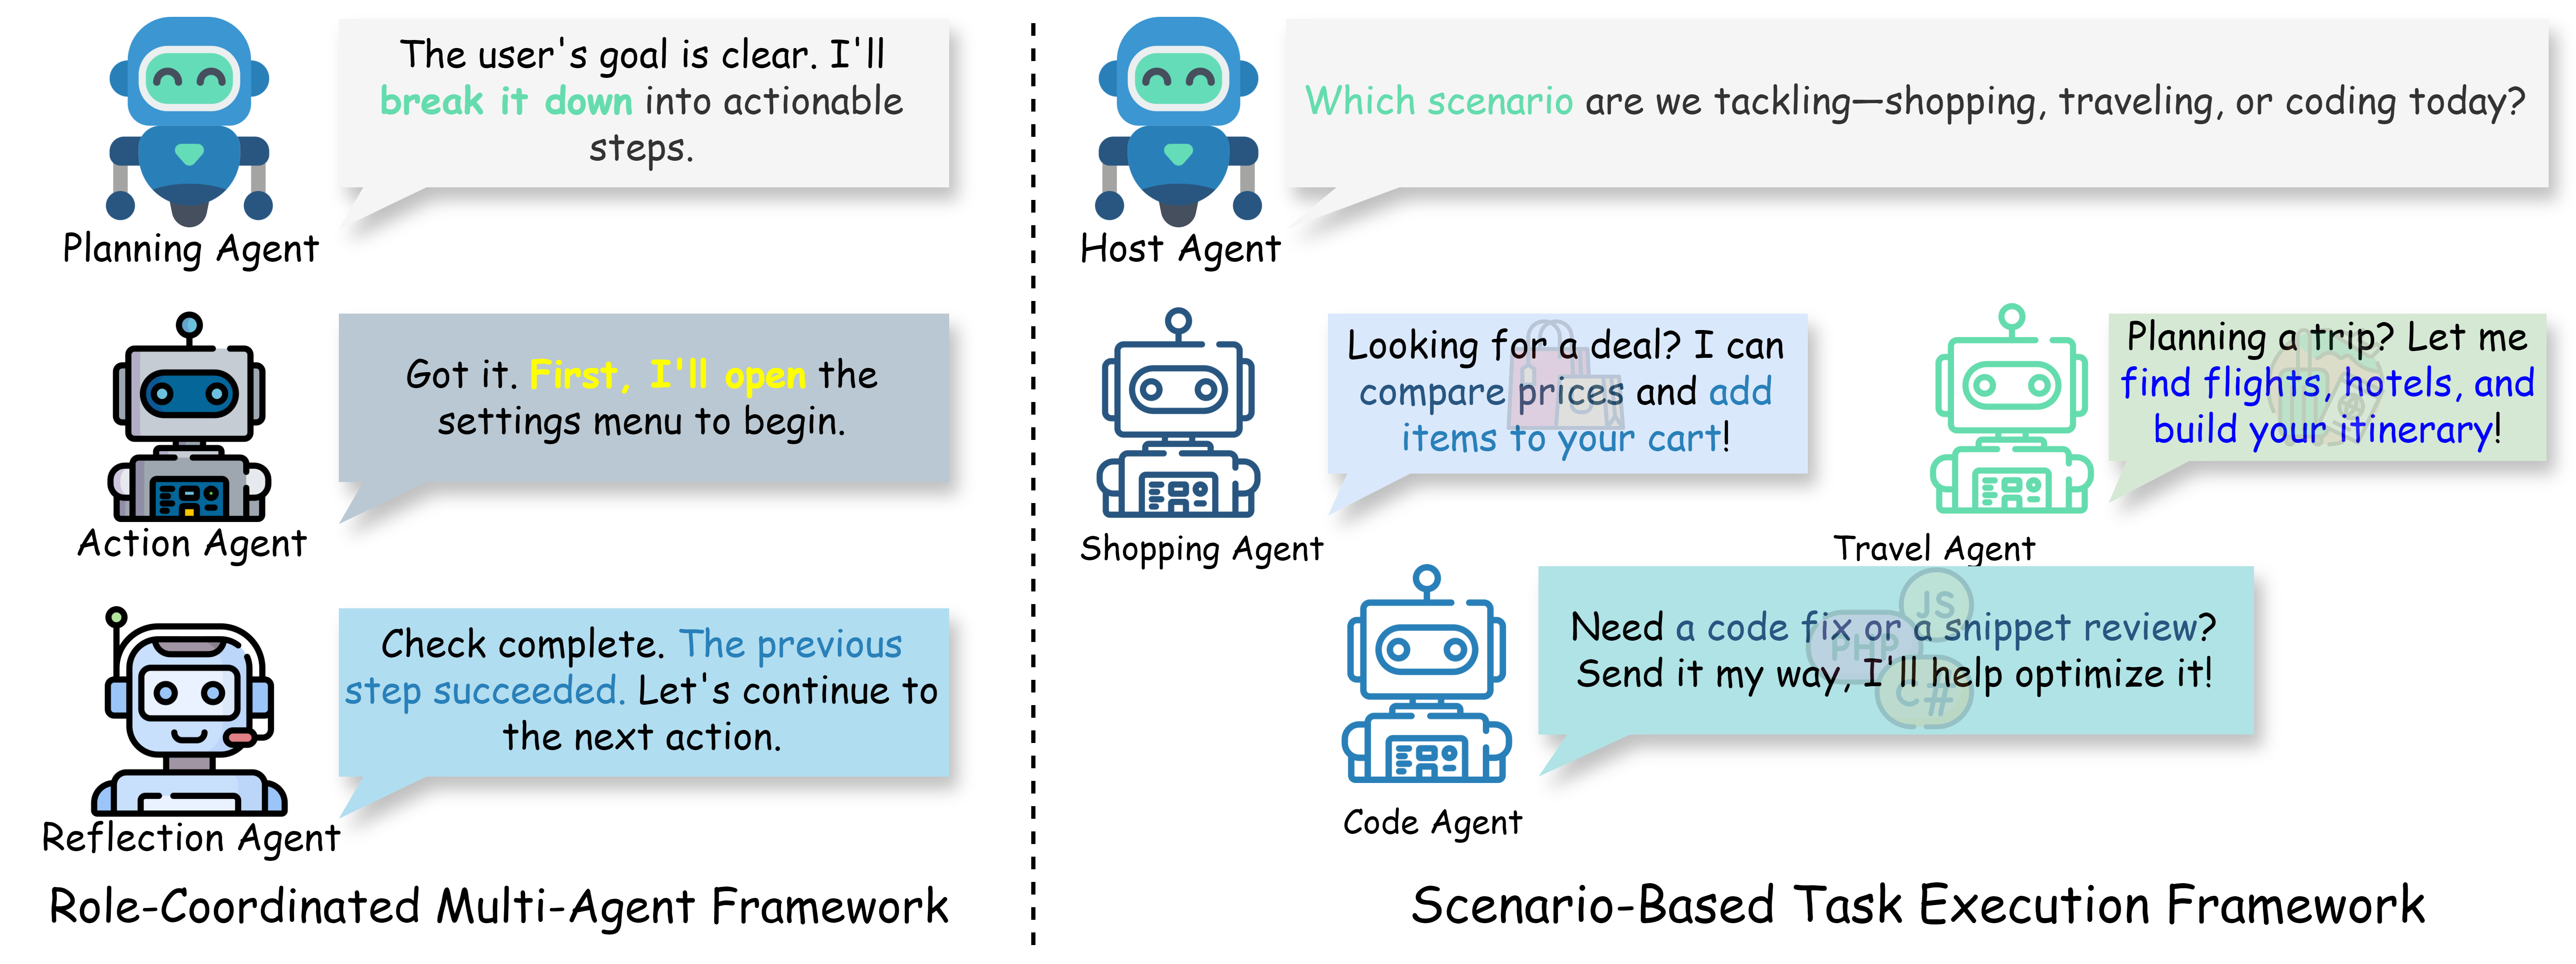
\includegraphics[width=0.95\textwidth]{figures/multi_agent_frameworks.drawio.png} \caption{Comparison of the role-coordinated and scenario-based multi-agent frameworks. The Role-Coordinated framework organizes agents based on general functional roles with a fixed workflow, while the Scenario-Based framework dynamically assigns tasks to specialized agents tailored for specific scenarios, allowing for increased flexibility and adaptability in handling diverse tasks.} \label{fig:multi_agent_frameworks} \end{figure*}


While single-agent frameworks based on LLMs have achieved significant progress in screen understanding and reasoning, they operate as isolated entities\cite{torreno2017cooperative,dorri2018multi,gong2023mindagent}. This isolation limits their flexibility and scalability in complex tasks that may require diverse, coordinated skills and adaptive capabilities. Single-agent systems may struggle with tasks that demand continuous adjustments based on real-time feedback, multi-stage decision-making, or specialized knowledge in different domains. Furthermore, they lack the ability to leverage shared knowledge or collaborate with other agents, reducing their effectiveness in dynamic environment~\cite{xi2023rise,wang2024mobileagentv2,tan2024cradle,song2024mmac}.

Multi-agent frameworks address these limitations by facilitating collaboration among multiple agents, each with specialized functions or expertise~\cite{chen2019control,talebirad2023multi,wu2023autogen,chen2023agentverse,li2023theory,liu2024dynamic,li2024survey,tran2025multi}. This collaborative approach enhances task efficiency, adaptability, and scalability, as agents can perform tasks in parallel or coordinate their actions based on their specific capabilities. As illustrated in Figure~\ref{fig:multi_agent_frameworks}, multi-agent frameworks in phone automation can be categorized into two primary types: the \textbf{Role-Coordinated Multi-Agent Framework} and the \textbf{Scenario-Based Task Execution Framework}. These frameworks enable more flexible, efficient, and robust solutions in phone automation by either organizing agents based on general functional roles or dynamically assembling specialized agents according to specific task scenarios.


\subsubsection{Role-Coordinated Multi-Agent}
\label{subsubsec: Role-Coordinated Multi-Agent}

In the Role-Coordinated Multi-Agent Framework, agents are assigned general functional roles such as planning, decision-making, memory management, reflection, or tool invocation. These agents collaborate through a predefined workflow, with each agent focusing on its specific function to collectively achieve the overall task. This approach is particularly beneficial for tasks that require a combination of these general capabilities, allowing each agent to specialize and optimize its role within the workflow.

For example, in MMAC-Copilot~\cite{song2024mmac}, multiple agents with distinct general functions collaborate as an OS copilot. The \textbf{Planner} strategically manages and allocates tasks to other agents, optimizing workflow efficiency. Meanwhile, the \textbf{Librarian} handles information retrieval and provides foundational knowledge, and the \textbf{Programmer} is responsible for coding and executing scripts, directly interacting with the software environment. The \textbf{Viewer} interprets complex visual information and translates it into actionable commands, while the \textbf{Video Analyst} processes and analyzes video content. Additionally, the \textbf{Mentor} offers strategic oversight and troubleshooting support. Each agent contributes its specialized function to the collaborative workflow, thereby enhancing the system's overall capability to handle complex interactions with the operating system.


Similarly, in Mobile-Agent-v2~\cite{wang2024mobileagentv2}, three agents with general roles are utilized: a planning agent, a decision agent, and a reflection agent. The \textbf{planning agent} compresses historical actions and state information to provide a concise representation of task progress. The \textbf{decision agent} uses this information to navigate the task effectively, while the \textbf{reflection agent} monitors the outcomes of actions and corrects any errors, ensuring accurate task completion. This role-based collaboration reduces context length, improves task progression, and enhances focus content retention through a memory unit managed by the decision agent.

In contrast, Mobile-Agent-E~\cite{wang2025mobile} decomposes tasks into high-level planning and low-level action execution, creating a system with a Manager Agent responsible for high-level planning and four subordinate agents: the Perceptor Agent, Operator Agent, Action Reflector Agent, and Notetaker Agent. The \textbf{Perceptor Agent} is responsible for fine-grained visual perception. The \textbf{Operator Agent} determines the next specific actions based on task and perception information. The \textbf{Action Reflector Agent} checks the screenshots before and after operations to verify if the expected outcomes are achieved and provides feedback to the Manager and Operator Agents. The \textbf{Notetaker Agent} extracts task-related information for use in subsequent steps. Additionally, Mobile-Agent-E incorporates a Self-Evolution Module, using two specialized agents, AES and AET, to update long-term memory after each task completion. \textbf{AES} summarizes lessons learned, while \textbf{AET} records reusable operational sequences, helping the agent in efficiently completing common subtasks and making better decisions in similar future tasks.



In general computer automation, Cradle~\cite{tan2024cradle} leverages foundational agents with general roles to achieve versatile computer control. Agents specialize in functions like command generation or state monitoring, enabling Cradle to tackle general-purpose tasks across multiple software environment.
Additionally, studies such as Ask-before-Plan~\cite{zhang2024ask}, PromptRPA~\cite{huang2024promptrpa}, LUMOS~\cite{yin2024agent}, and WebPilot~\cite{zhang2024webpilot} also utilize general-purpose role agents to execute tasks and excel in complex tasks like planning. Among these, LUMOS provides high-quality training data and methods for future intelligent agent research.


\subsubsection{Scenario-Based Task Execution}
\label{subsubsec: Scenario-Based Task Execution}

In the Scenario-Based Task Execution Framework, tasks are dynamically assigned to specialized agents based on specific task scenarios or application domains. Each agent is endowed with capabilities tailored to a particular scenario, such as shopping, code editing, or navigation. By assigning tasks to agents specialized in the relevant domain, the system improves task success rates and efficiency.

For instance, MobileExperts~\cite{zhang2024mobileexperts} forms different expert agents through an \textbf{Expert Exploration phase}. In the exploration phase, each agent receives tailored tasks broken down into sub-tasks to streamline the exploration process. Upon completion of a sub-task, the agent extracts three types of memories from its trajectory: interface memories, procedural memories (tools), and insight memories for use in subsequent execution phases. When a \textbf{new task} arrives, the system dynamically forms an expert team by \textbf{selecting agents whose expertise matches the task requirements}, enabling them to collaboratively execute the task more effectively. Similarly, in the SteP~\cite{sodhi2024step} framework, agents are specialized based on \textbf{specific web scenarios} such as shopping, GitLab, maps, Reddit, or CMS platforms. Each scenario agent possesses specific capabilities and knowledge relevant to its domain. When a task is received, it is dynamically assigned to the appropriate scenario agent, which executes the task leveraging its specialized expertise. This approach enhances flexibility and adaptability, allowing the system to handle a wide range of tasks across different domains more efficiently.

Through dynamic task assignment and specialization, the Scenario-Based Task Execution Framework optimizes multi-agent systems to adapt to diverse and evolving contexts, significantly enhancing both the efficiency and effectiveness of task execution. As illustrated in Figure~\ref{fig:multi_agent_frameworks}, the Role-Coordinated Framework relies on agents with general functional roles collaborating through a fixed workflow, suitable for tasks requiring a combination of general capabilities. In contrast, the Scenario-Based Framework dynamically assigns tasks to specialized agents tailored to specific scenarios, providing a flexible structure that adapts to the varying complexity and requirements of real-world tasks.


Despite the potential of multi-agent frameworks in phone automation, several challenges remain. In the Role-Coordinated Framework, coordinating agents with general functions requires efficient workflow design and may introduce overhead in communication and synchronization. In the Scenario-Based Framework, maintaining and updating a diverse set of specialized agents can be resource-intensive, and dynamically assigning tasks requires effective task recognition and agent selection mechanisms. Future research could explore hybrid frameworks that combine the strengths of both approaches, leveraging general functional agents while also incorporating specialized scenario agents as needed. Additionally, developing advanced algorithms for agent collaboration, learning, and adaptation can further enhance the intelligence and robustness of multi-agent systems. Integrating external knowledge bases, real-time data sources, and user feedback can also improve agents' decision-making capabilities and adaptability in dynamic environment.

\begin{figure*}[ht] 
    \centering 
    \includegraphics[width=0.95\textwidth]{figures/model_differences.drawio.png} 
    \caption{Differences between training-based methods and prompt engineering in phone automation. Training-based methods adapt the model's parameters through additional training, enhancing its ability to perform specific tasks, whereas prompt engineering leverages the existing capabilities of pre-trained models by guiding them with well-designed prompts. } 
    \label{fig:model_differences} 
\end{figure*}

\subsection{Plan-Then-Act Framework}
\label{subsec:plan_then_act}

While single-agent and multi-agent frameworks enhance adaptability and scalability, some tasks benefit from explicitly separating high-level planning from low-level execution. This leads to what we term the \textit{Plan-Then-Act Framework}. In this paradigm, the agent first formulates a conceptual plan—often expressed as human-readable instructions—before grounding and executing these instructions on the device’s UI.

The Plan-Then-Act approach addresses a fundamental challenge: although LLMs and multimodal LLMs (MLLMs) excel at interpreting instructions and reasoning about complex tasks, they frequently struggle to precisely map their textual plans to concrete UI actions. By decoupling these stages, the agent can focus on \textbf{\emph{what} should be done (planning)} and then handle \textbf{\emph{how} to do it on the UI (acting)}. Recent works highlight the effectiveness of this approach:

\noindent$\bullet$ SeeAct~\cite{zheng2024gpt} demonstrates that GPT-4V(ision)\cite{achiam2023gpt} can generate coherent plans for navigating websites. However, bridging the gap between textual plans and underlying UI elements remains challenging. By clearly delineating planning from execution, the system can better refine its plan before finalizing actions.

\noindent$\bullet$ UGround~\cite{gou2024navigating} and related efforts~\cite{you2024ferret,zhang2024ui-hawk} emphasize advanced visual grounding. Under a Plan-Then-Act framework, the agent first crafts a task solution plan, then relies on robust visual grounding models to locate and manipulate UI components. This modular design enhances performance across diverse GUIs and platforms, as the grounding model can evolve independently of the planning mechanism.

\noindent$\bullet$ LiMAC (Lightweight Multi-modal App Control)~\cite{christianos2024lightweight} also embodies a Plan-Then-Act spirit. LiMAC’s Action Transformer (AcT) determines the required action type (the plan), and a specialized VLM is invoked only for natural language needs. By structuring decision-making and text generation into distinct stages, LiMAC improves responsiveness and reduces compute overhead, ensuring that reasoning and UI interaction are cleanly separated.

\noindent$\bullet$ ClickAgent~\cite{hoscilowicz2024clickagent} similarly employs a two-phase approach. The MLLM handles reasoning and action planning, while a separate UI location model pinpoints the relevant coordinates on the screen. Here, the MLLM’s plan of which element to interact with is formed first, and only afterward is the element's exact location identified and the action executed.

\noindent$\bullet$ Ponder \& Press~\cite{wang2024ponder} employs a general MLLM to decompose user instructions into executable actions. It then uses a GUI-specific MLLM to map the target elements in the action descriptions to pixel coordinates, thereby constructing a Plan-Then-Act Framework based solely on visual input. This framework is adaptable across various software environments without relying on supplementary information such as HTML or UI Trees.

% Ponder \& Press 利用通用MLLM将用户指令分解为可执行动作,随后使用GUI特定MLLM作为将动作描述中的目标元素定位到像素坐标,实现仅通过视觉输入构建 Plan-Then-Act Framework。该框架能够在多种软件环境中灵活应用,无需依赖HTML、UI Tree等辅助信息。

The Plan-Then-Act Framework offers several advantages. Modularity allows improvements in planning without requiring changes to the UI grounding and execution modules, and vice versa. Error Mitigation enables the agent to revise its plan before committing to actions; if textual instructions are ambiguous or infeasible, they can be corrected, reducing wasted actions and improving reliability. Additionally, improved visual grounding models, OCR enhancements, and scenario-specific knowledge can further refine the Plan-Then-Act approach, making agents more adept at handling intricate, real-world tasks.
In summary, the Plan-Then-Act Framework represents a natural evolution in designing MLLM-powered phone GUI agents. By separating planning from execution, agents can achieve clearer reasoning, improved grounding, and ultimately more effective and reliable task completion.